%!TEX root = main.tex

\newpage
\chapter{Informačné bulletiny}

Informačné bulletiny (angl. \emph{newsletters}) sú aj v súčasnosti jedným z najrozšírenejších spôsobov, ako v online
prostredí informovať používateľov o dianí na webovom portáli. Prevádzkovatelia webových portálov využívajú informačné
bulletiny na predstavenie nového obsahu, akciového tovaru, zaujímavostí z určitej oblasti alebo špeciálnych ponúk pre
svojich používateľov a zákazníkov. Informačné bulletiny sú tiež využívané ako prostriedok pre motiváciu používateľov
k opätovnej návšteve webového portálu.

Informačné bulletiny spravidla nadobúdajú formu e-mailu, ktorý je zvyčajne v pravidelných intervaloch doručovaný
do schránok používateľov, ktorí o jeho doručovanie prejavili záujem.


\section{Problémy informačných bulletinov}
Hlavným problémom informačných bulletinov v súčasnosi je stále sa znižujúva miera interakcie používateľov
s informačnými bulletinmi.

Štúdia spoločnosti Silverpop z roku 2012~\cite{mailmarketing} na vzorke informačných bulletinov 1124 spoločností ukázala,
že počet používateľov, ktorí vôbec otvoria informačný bulletin sa pohybuje na úrovni 20\% a stále klesá. Navyše konkrétne
v oblasti technológií sa táto hodnota pohybuje len na 16,5\%. Ešte menšia je miera preklikov
(angl. \emph{Click-through rate - CTR}), ktorá sa celkovo pohybuje na úrovni 5,4\% a v prípade technologicky zameraných
informačných bulletinov len 3,6\%. Napriek tomu sa miera odhlásení z odoberania (angl. \emph{unsubscribe rate}) pohybuje
len na úrovni 2\%.

Dôvodov, prečo používatelia prejavujú iba malý záujem o informačné bulletiny ktoré im sú doručované, môže byť niekoľko.
Jedným z takýchto dôvodov môže byť vysoká saturácia -- používateľom chodí priveľké množstvo informačných bulletinov,
dôsledkom čoho používatelia rezignujú a tieto e-maily ani neotvárajú.
Hlavným nedostatkom informačných bulletinov, a zároveň dôvodom, prečo iba 5\% používateľov klikne na obsah v informačnom
bulletine, je však relevancia ponúkaného obsahu.


\section{Relevancia v informačných bulletinoch}

Množstvo webových portálov doručuje všetkým svojim používateľom presne ten istý obsah informačného bulletinu.
Často je tento obsah vytváraný manuálne editormi, a zameriava sa len všeobecne na aktuálne dianie na danom webovom
portáli. Takýto všeobecný informačný bulletin však nutne nemôže byť dostatočne relevantný pre značnú časť používateľov.

Riešením problému relevancie infromačných bulletinov je vytváranie personalizovaných informačných bulletinov, ktoré
každému používateľovi ponúkajú len ten obsah, ktorý je pre neho najzaujímavejší a najrelevantnejší.


\section{Informačné bulletiny v CQA systémoch}

Význam informačných bulletinov značne narastá aj v rámci online komunít, ktoré produkujú veľké množstvo používateľmi
vytváraného obsahu. Medzi prominentné druhy takýchto online komunít patria aj systémy pre odpovedanie na otázky
(angl.~\emph{Community Question Answering - CQA}).

Súčasný výskum v oblasti CQA systémov~\cite{Srba2016} sa venuje predovšetkým oblastiam skúmania správania používateľov,
smerovania a odporúčania otázok a kvality otázok a odpovedí v týchto systémoch. Problematike vytvárania informačných
bulletinov v doméne CQA systémov zatiaľ nebola venovaná veľká pozornosť.

Mnohé populárne CQA systémy aj v súčasnosti ponúkajú svojim používateľom informačné bulletiny majúce iba generický
charakter a nijakým spôsobom neuvažujú relevantnosť obsahu pre konkrétnych používateľov, prípadne informačné bulletiny
neponúkajú vôbec.

\subsection{Informačné bulletiny v sieti Stack Exchange}

Sieť Stack Exchange\footnote{\url{https://stackexchange.com}}, ktorá patrí medzi najpopulárnejšie CQA systémy súčasnosti,
sa skladá z viac ako 160 samostatných komunít zameraných na rôzne oblasti. Stack Exchange ponúka používateľom všetkých
komunít možnosť odoberať informačný bulletin, ktorý je doručovaný raz týždenne.

Informačné bulletiny komunít Stack Exchange obsahujú tri sekcie (Obr.~\ref{fig:so-newsletter}). Prvá sekcia je rovnaká
pre všetkých používateľov konkrétnej komunity a obsahuje zoznam najlepšie hodnotených nových otázok.
Obsah nasledujúcich dvoch sekcií je náhodne generovaný. Tieto sekcie obsahujú najpopulárnejšie otázky z predchádzajúceho
týždňa a náhodný výber nezodpovedaných otázok.

Používatelia CQA systému Stack Exchange nie sú s takýmto generickým informačným bulletinom
spokojní~\cite{so-meta-newsletter}. Generický informačný bulletin stráca pre používateľov informačnú hodnotu, pretože
najmä v prípade väčších komunít, akou je napríklad Stack Overflow\footnote{\url{https://stackoverflow.com}}, často obsahuje
otázky, ktoré nie sú z oblastí záujmu používateľa. Najviac sa tento problém prejavuje na sekcii nezodpovedaných otázok.
Tie sú vyberané náhodne, takže pravdepodobnosť, že používateľ vie na niektorú z nich odpovedať, je malá.

\begin{figure}[H]\begin{center}
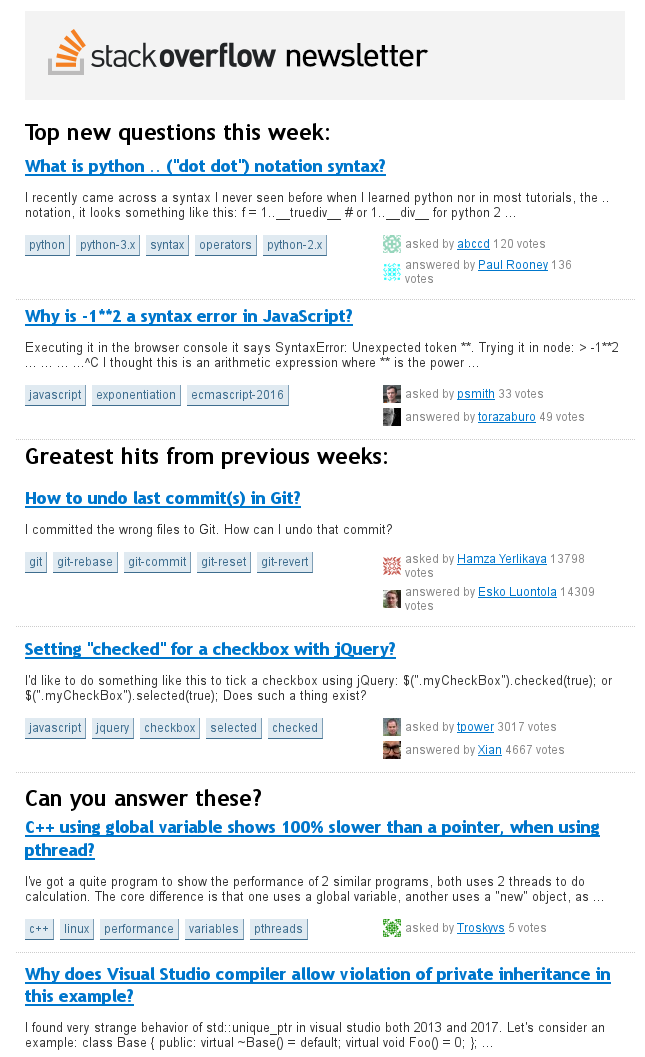
\includegraphics[scale=0.4]{so-newsletter}
\caption{Informačný bulletin komunity Stack Overflow, 25. apríl 2017.\label{fig:so-newsletter}}\end{center}
\end{figure}

\subsection{Informačný bulletin portálu Quora}

Quora\footnote{\url{https://quora.com}} je CQA systém, ktorý nie je zameraný na konkrétnu oblasť záujmu, ale obsahuje
otázky z rôznych tém. Quora ponúka svojim používateľom týždenný informačný bulletin (\emph{Quora Weekly Digest}),
ktorý obsahuje desať najzaujímavejšich otázok za posledný týždeň a zoznam ľudí, ktorých používateľ potenciálne pozná.

Zoznam najzaujímavejších otázok pozostáva z editormi manuálne vybraného obsahu a algoritmicky vybraného obsahu,
ktorý je personalizovaný pre každého používateľa zvlášť (Obr.~\ref{fig:quora-newsletter}).

\begin{figure}[H]\begin{center}
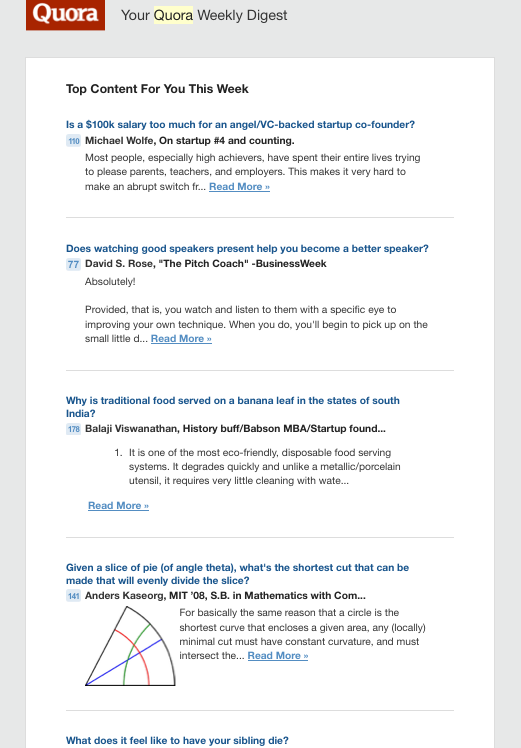
\includegraphics[scale=0.5]{quora-newsletter}
\caption{Informačný bulletin portálu Quora. Prevzaté 30.4.2017, \url{http://www.businessinsider.com/quora-emails-2012-8}
\label{fig:quora-newsletter}}\end{center}
\end{figure}

\subsection{CQA systémy bez informačných bulletinov}

Viaceré populárne CQA systémy svojim používateľom vôbec neponúkajú možnosť odoberať informačný bulletin. Medzi takéto
systémy patrí napr. portál \emph{Yahoo! Answers}\footnote{\url{https://answers.yahoo.com}}, ktorý je určený na pokladanie
otázok z akejkoľvek oblasti záujmu. Rovnako informačný newsletter neponúka ani ďalší všeobecne zameraný CQA systém --
\emph{Wiki Answers}\footnote{\url{https://answers.com}}. CQA systém zameraný na podporu výučby
\emph{Askalot}\footnote{\url{http://askalot.fiit.stuba.sk}} tiež v súčasnosti neponúka informačný newsletter,
iba možnosť notifikácie používateľa prostredníctvom e-mailu o aktivite súvisiacej s jeho obsahom v rámci systému.



%%%%%%%%%%%%%%%%%%%%%%%%%%%%%%%%%%%%%%%%%%%%%%%%%%%%%%%%%%%%%%%%%%%%%%%%%%%%%%%%%%%%%%%%%%%%%%%%%%%%%%%%%%%%%%%%%%%%%%%%


\newpage
\chapter{CQA systémy}

CQA systémy sú jednou z výrazných skupín webových portálov, ktoré sú založené na princípe používateľsky vytváraného obsahu.
Tieto systémy umožňujú používateľom položiť otázky, ktoré nie je možné zodpovedať použitím štandardných vyhľadávačov~\cite{Liu2012}
a zároveň odpovedať na otázky iných používateľov.

Napriek tomu, že väčšina CQA systémov sa spočiatku zameriava najmä na poskytnutie zmysluplnej odpovede na konkrétnu otázku,
v súčasnosti je možné v prípade niektorých CQA systémov (napr. Stack Overflow) vnímať postupnú zmenu zamerania
z jednorázových odpovedí na kolaboratívne vytváranie komplexnejších poznatkov s dlhodobou hodnotou~\cite{Anderson2012}.
Za týmto účelom CQA systémy implementujú hlasovanie a princíp reputácie ako spôsob podpory komunitného aspektu označovania
najlepších odpovedí na položené otázky.


\section{Problémy CQA systémov}

CQA systémy sa musia vysporiadavať s tými istými druhmi problémov, ako iné kategórie systémov založené na používateľmi
vytvorenom obsahu.

\subsection{Problém dlhého chvosta}
Čím viac sa zvýrazňuje trend orientácie CQA systémov viac na poskytovanie obsahu s dlhodobou hodnotou ako na samotné
poskytnutie odpovede na položenú otázku, tým viac sa prehlbuje problém \emph{dlhého chvosta} (angl. \emph{long tail}).
Ide o štandardný problém všetkých stránok zameriavajúcich sa na používateľmi vytváraný obsah, kedy je veľká väčšina
používateľov týchto stránok len pasívnymi čitateľmi (angl. \emph{lurkers}) a najväčšia časť obsahu je vytvorená len veľmi
úzkou skupinou najaktívnejších používateľov.

V prípade CQA systému Stack Overflow sa podiel aktívnych používateľov (takých, ktorí za sledovaný mesiac pridali
do systému aspoň jednu otázku alebo odpoveď) za marec 2017 pohyboval na úrovni 3\% všetkých
používateľov~\cite{Srba2016SOFail}\footnote{Výsledky za aktuálne obdobie boli získané prostredníctvom nástroja Stack
Exchange Data Explorer.}.

\subsection{Variabilita v kvalite obsahu}
Ďalším problémom CQA systémov je variabilná kvalita otázok a odpovedí v týchto systémoch. Zvyšujúcou sa popularitou CQA
systémov narastá aj podiel obsahu s nízkou kvalitou, či už vo forme veľmi jednoduchých otázok alebo nedostatočne
podrobných odpovedí, ako aj množstvo duplicitných otázok -- otázok, ktoré už boli v systéme
zodpovedané~\cite{Srba2016SOFail}\cite{Ponzanelli2014}.

Jedným z riešení tohto problému, ktorý využíva aj CQA systém Stack Overflow, je komunitné zabezpečovanie kvality obsahu
prostredníctvom moderátorov -- používateľov s oprávnením upravovať, označiť duplikát alebo vymazať obsah.


\section{Druhy CQA systémov}

CQA systémy možno kategorizovať do dvoch základných skupín podľa toho, na akú oblasť otázok sa tieto systémy zameriavajú.

\subsection{Univerzálne CQA systémy}

CQA systémy ako \emph{Yahoo! Answers}, \emph{Wiki Answers} alebo \emph{Quora} nie sú zamerané na konkrétne oblasti
a umožňujú používateľom pokladať otázky na akékoľvek témy~\cite{Chua2014}.

Tento druh CQA systémov má štandardne vyšší počet používateľov aj aktivity ako úzko špecializované CQA systémy,
no tiež tu existuje väčšia pravdepodobnosť výskytu nekvalitných, jednoduchých alebo neužitočných otázok a odpovedí,
ako aj veľký počet duplicitných otázok, ktoré už boli zodpovedané. Zároveň sú univerzálne CQA systémy zameriané viac
na samotný proces kladenia otázok a odpovedania na ne, než na vytváranie dlhodobo hodnotného obsahu.

\subsection{Úzko špecializované CQA systémy}

Opakom univerzálnych CQA systémov sú CQA systémy, ktoré sú špecializované na konkrétne oblasti záujmu.
Medzi takéto CQA systémy patria napríklad jednotlivé komunity v rámci siete Stack Exchange, ktorá zahŕňa rôzne druhy
komunít, od všeobecnejších, ako je napr. komunita venujúca sa matematike\footnote{\url{https://math.stackexchange.com}},
po veľmi úzko špecializované, akými sú napr. komunity \emph{Ask Ubuntu}\footnote{\url{https://askubuntu.com}} alebo
\emph{Raspberry Pi}\footnote{\url{https://raspberrypi.stackexchange.com}} venujúce sa konkrétnym produktom.

Tématicky zamerané CQA systémy majú väčší potenciál pre vznik dlhodobo hodnotného obsahu~\cite{Anderson2012}. V rámci
týchto systémov tiež vzniká množstvo prepojení medzi obsahom \textit{(otázky podobného charakteru, riešenie problému
v príbuznej oblasti)}, čo vedie k vzniku \emph{znalostných sietí}~(angl.~\emph{knowledge networks})~\cite{Li2016}.
S cieľom zvýšiť hodnotu jednotlivých príspevkov tiež mnohé CQA systémy zavádzajú možnosť komunitnej úpravy
otázok a odpovedí~\cite{Li2015}, čo vedie okrem zvýšenej aktivity aj k zvýšeniu vnímanej užitočnosti príspevku.



%%%%%%%%%%%%%%%%%%%%%%%%%%%%%%%%%%%%%%%%%%%%%%%%%%%%%%%%%%%%%%%%%%%%%%%%%%%%%%%%%%%%%%%%%%%%%%%%%%%%%%%%%%%%%%%%%%%%%%%%


\chapter{Odporúčanie}

\section{Odporúčacie systémy}

Odporúčacie systémy sú softvérové nástroje a techniky ktoré používateľom ponúkajú položky, ktoré by pre nich mohli
byť nejakým spôsobom zaujímavé alebo užitočné~\cite{Handbook2011}. Tieto odporúčania sú zvyčajne ponúkané za účelom
pomôcť používateľovi rozhodnúť sa, aké články by si mal prečítať, alebo aký tovar si kúpiť.

Využívanie odporúčacích systémov je tiež pre používateľov vhodným spôsobom, ako zvládať problémy informačného zahltenia
v dnešnom online svete. Ako také sa odporúčacie systémy stávajú jedným z najsilnejších a najpopulárnejších nástrojov
v online komunitách.

Odporúčacie systémy typicky vytvárajú zoznam odporúčaní jedným z dvoch spôsobov -- buď prostredníctvom \emph{kolaboratívneho
filtrovania} (angl.~\emph{Collaborative filtering}), alebo použitím \emph{filtrovania založeného na obsahu}
(angl.~\emph{Content-based filtering})~\cite{Buhmann2011}. Tieto dva prístupy môžu byť tiež kombinované
v hybridných odporúčacích systémoch.

\subsection{Kolaboratívne filtrovanie}

Odporúčacie systémy využívajúce kolaboratívne filtrovanie fungujú prostredníctvom získavania spätnej väzby používateľa
vo forme hodnotení pre položky v danej doméne a využívajú podobnosti v hodnotení medzi viacerými používateľmi na určenie
či určitý obsah odporučiť, alebo nie~\cite{Buhmann2011}. Metódy kolaboratívneho filtrovania možno ďalej rozdeliť
na metódy založené na susednosti alebo na základe modelu.

Kolaboratívne filtrovanie na základe susednosti (angl.~\emph{Neighborhood-based Collaborative filtering})
vyberá skupinu používateľov podľa ich podobnosti k aktuálnemu používateľovi
a použitím váženej kombinácie ich hodnotení vyberá odporúčaný obsah pre tohto používateľa.
Techniky založené na modeli (angl.~\emph{Model-based Collaborative filtering}) poskytujú odporúčania prostedníctvom
oceňovania parametrov štatistických modelov pre používateľské hodnotenia.

\subsection{Filtrovanie na základe obsahu}

Odporúčanie čisto prostedníctvom kolaboratívneho filtrovania využíva iba používateľské hodnotenia. Tieto prístupy berú
všetkých používateľov a položky ako atomické jednotky a odporúčania sú vytvárané bez ohľadu na konkrétne špecifiká
individuálnych používateľov alebo položiek.

Metódy využívajúce filtrovanie na základe obsahu naopak vytvárajú
odporúčania na základe porovnávania modelov reprezentujúcich obsah s modelmi reprezentujúcimi konkrétneho používateľa.
Odporúčania v takýchto prístupoch vznikajú na základe prekryvu týchto dvoch modelov.


\section{Odporúčanie v CQA systémoch}



- Odporucanie v CQA systemoch
- Question Routing, Question recommendation, retrieval... definitions...
- Challenges:
    - Cold start
    - Filter bubble



%%%%%%%%%%%%%%%%%%%%%%%%%%%%%%%%%%%%%%%%%%%%%%%%%%%%%%%%%%%%%%%%%%%%%%%%%%%%%%%%%%%%%%%%%%%%%%%%%%%%%%%%%%%%%%%%%%%%%%%%


\chapter{Diverzifikácia a aktuálnosť}

- Diverzifikacia v odporucacich systemoch -> riesenie filter bubble
- Dopad aktualnosti na uspesnost odporucania
- D and A v CQA
